\section{Three-flavor \chpt\ to leading order}
\label{section: three-flavor chpt to leading order}

For $N_f = 3$, the generators are $T_\alpha = \frac{1}{2} \lambda_\alpha$, where $\lambda_\alpha$ are the Gell-Mann matrices, as shown in \autoref{section: algebra bases}.
The vacuum parametrization of the Goldstone bosons is
%
\begin{equation}
    \Sigma(x) = \exp{i\frac{\varphi_a \lambda_a}{f}}.
\end{equation}
%
The $\varphi_a$-fields, of which there are eight, are related to the observed pseudoscalar mesons by~\autocite{schererIntroductionChiralPerturbation2002}
%
\begin{equation}
    \varphi_a \lambda_a
    =
    \begin{pmatrix}
        \varphi_3 + \frac{1}{\sqrt{3}} \varphi_8 & \varphi_1 - i \varphi_2 & \varphi_4 - i \varphi_5 \\
        \varphi_1 + i \varphi_2 & \varphi_3 + \frac{1}{\sqrt{3}} \varphi_8 & \varphi_6 - i \varphi_7  \\
        \varphi_4 - i \varphi_5 & \varphi_6 - i \varphi_7  & \frac{2}{\sqrt{3}} \varphi_8
    \end{pmatrix}
    =
    \begin{pmatrix}
        \pi_0 + \frac{1}{\sqrt{3}}\eta & \sqrt{2}\pi^+ & \sqrt{2}K^+ \\
        \sqrt{2}\pi^- & -\pi_0 + \frac{1}{\sqrt{3}}\eta & \sqrt{2}K^0 \\
        \sqrt{2}K^- & \sqrt{2}\bar K^0  & - \frac{2}{\sqrt 3} \eta
    \end{pmatrix}.
\end{equation}
%
The mass matrix is now
%
\begin{equation}
    m = 
    \begin{pmatrix}
        m_u & 0 & 0 \\
        0 & m_d & 0 \\
        0 & 0 & m_s
    \end{pmatrix},
\end{equation}
%
To include this in the effective Lagrangian, we define
%
\begin{equation}
    \chi = 2B_0 m = 
    \begin{pmatrix}
        \bar m^2 - \Delta m^2 & 0 &0\\
        0& \bar m^2 + \Delta m^2 & 0 \\
        0&0&m_S^2
    \end{pmatrix},
\end{equation}
%
where
%
\begin{equation}
    \bar m^2 =  B_0(m_u + m_d),\quad 
    \Delta m^2 = B_0(m_d - m_u), \quad
    m_S^2 = 2B_0 m_s.
\end{equation}
%
The charge matrix is
%
\begin{equation}
    \label{three-flavor charge matrix}
    Q = \frac{1}{3}
    \begin{pmatrix}
        2 & 0 & 0\\
        0 & -1 & 0\\
        0 & 0 & -1
    \end{pmatrix}
    = \frac{1}{2} \left( \lambda_3 + \frac{1}{\sqrt{3}} \lambda_8 \right).
\end{equation}
%
The leading order Lagrangian has the same form as for $\Lie{SU}{2}$,
%
\begin{equation}
    \label{leading order three-flavor lagrangian}
    \Ell_2 
    = \frac{1}{4}f^2 \Tr{\nabla_\mu \Sigma \nabla^\mu \Sigma^\dagger}
    + \frac{1}{4}f^2 \Tr{\chi \Sigma^\dagger + \Sigma \chi^\dagger}
    + e^2 C \Tr{\Sigma Q \Sigma^\dagger Q}.
\end{equation}
%


\subsection{Ground state}

We will start the analysis by assuming $e = 0$ and then reintroduce electromagnetic interactions later.
The covariant derivative is then
%
\begin{equation}
    \nabla_\mu \Sigma = \partial_\mu \Sigma - i [v_\mu, \Sigma], \quad 
    v_\mu = \mu \delta^0_\mu,
\end{equation}
%
Here, $\mu$ is the chemical potential matrix,
%
\begin{equation}
    \mu = 
    \begin{pmatrix}
        \mu_u & 0 & 0 \\
        0 & \mu_d & 0 \\
        0 & 0 & \mu_s
    \end{pmatrix}
    = 
    \begin{pmatrix}
        \frac{1}{3}\mu_B + \frac{1}{2}\mu_I & 0 & 0 \\
        0 & \frac{1}{3}\mu_B - \frac{1}{2}\mu_I & 0 \\
        0 & 0 & \frac{1}{3}\mu_B - \mu_S
    \end{pmatrix}
    = \frac{1}{3}(\mu_B - \mu_S) \one 
    + \frac{1}{2} \mu_I \lambda_3
    + \frac{1}{\sqrt{3}}\mu_S\lambda_8,
\end{equation}
%
where $\mu_B = \frac{3}{2}(\mu_u + \mu_d)$, $\mu_I = \mu_u - \mu_d $ and $\mu_S = \frac{1}{2}(\mu_u + \mu_d)-\mu_s$.
Here, $\mu_u$, $\mu_d$, and $\mu_s$ are the up, down, and strange quark chemical potentials, while $\mu_B$, $\mu_I$, and $\mu_S$ are the baryon number, isospin, and strangeness chemical potentials.
The baryon number of mesons, and thus the $\pi_a$'s, is zero.
Consequently, $\Sigma$ transforms as $\Sigma \rightarrow \Sigma$ under $U(1)_V$, the symmetry corresponding to the baryon number; it is a baryon number singlet.
Therefore, the chemical potential corresponding to the baryon number, $\mu_B$, should not affect the final result.
We can also see this because $\mu_B$ only appears with the identity matrix $\one$ in $\mu$.
Any dependence on $\mu_B$ in $\nabla_\mu \Sigma$ will vanish as $\one$ commutes with everything.

The $\lie{su}{3}$ Lie algebra has three independent $\lie{su}{2}$ sub-algebras.
We introduce the matrices
%
\begin{equation}
    \lambda_Q = \lambda_3 + \frac{1}{\sqrt{3}}\lambda_8, \quad
    \lambda_K = \lambda_3 - \frac{1}{\sqrt{3}}\lambda_8,
\end{equation}
%
From the structure constants, \autoref{structure constants su(3)}, we can conclude that they commute, i.e., $[\lambda_Q, \lambda_K] = 0$.
Furthermore, we find the commutation relations
%
\begin{equation}
    [\lambda_i, \lambda_j] = 2i \epsilon_{ijk} \lambda_k,\quad
    ijk \in
    \begin{cases}
        &\{1, 2, 3\}\\ &\{4, 5, Q\}\\ &\{6, 7, K\}.
    \end{cases}
\end{equation}
%
We here define the Levi-Civita symbol by $\epsilon_{123} = \epsilon_{34Q} =\epsilon_{76K} = 1$. \todo[]{Dobbeltsjekk rekkefølge på 76K}
This is the defining commutation relation of $\lie{su}{2}$.
To find the ground state, we define
%
\begin{equation}
    \Sigma_\alpha 
    = \exp{i \alpha n_a \lambda_a},
    \quad \alpha = \frac{1}{f} \sqrt{\varphi_a^0 \varphi_a^0}, \quad n_a = \frac{\varphi_a^0}{\sqrt{\varphi_b^0 \varphi_b^0}}. 
\end{equation}
%
For $\mu_S = 0$, we expect to recover the results from the two-flavor case, which corresponds to $n_1^2 + n_2^2 =1$, $n_a = 0$ for $i>2$.
As argued earlier, we may choose $n_1 = 0$ without loss of generality, in which case the ground state becomes
%
\begin{equation}
    \Sigma_\alpha^{\pipm} = \exp{i \alpha \lambda_2} = (\one - \lambda^2_2) + \lambda_2^2 \cos\alpha + i \lambda_2\sin\alpha.
\end{equation}
%
If we define $\mu_\Kpm = (\frac{1}{2}\mu_I + \mu_S)$ and $\mu_\Ko = (\frac{1}{2}\mu_I - \mu_S)$, then we can write the external currents corresponding to $\mu_I$ and $\mu_S$ as
%
\begin{equation}
    \frac{1}{2}\mu_I \lambda_3 + \frac{1}{\sqrt 3}\mu_S \lambda_8 = \frac{1}{2}\mu_\Kpm \lambda_Q + \frac{1}{2} \mu_\Ko \lambda_K.
\end{equation}
%
Analogously to how turning up $\mu_I$ leads to a condensate in the first $\lie{su}{2}$ subalgebra, we can expect these chemical potentials to lead to different condensates in their respective subalgebras.
If we assume $\mu_\Ko = 0$, we would expect the new ground state to take the form
%
\begin{align}
    \Sigma_\alpha^{\Kpm} = \exp{i \alpha \lambda_5} = (\one - \lambda^2_5) + \lambda_5^2 \cos\alpha + i \lambda_5\sin\alpha.
\end{align}
%
This analysis extends to all four quadrants of the $\mu_I-\mu_S$ plane.
If we set $\mu_\Kpm = 0$, we would expect a ground state of the form $e^{i\alpha\lambda_7}$.
In \autocite{kogutQCDSmallNonzero2001}, \citeauthor{kogutQCDSmallNonzero2001} show that exactly this happens. 
At $\mu_\Kpm^2 \geq m_K^2 = \bar m + m_S(+\Delta m?)$, we get a charged pion condensate, and a neutral kaon condensate at $\mu_\Ko^2 \geq m_K^2$.\todo[]{skal det egt. være $m_\Kpm$ og $m_\Ko$?}
However, the domains of the different condensates overlap, so there is a phase transition between the condensates.
\todo[]{Find the criterion for phase transition between the condensates}
\autoref{fig: phase diagram} shows the phase diagram in the $\mu_I-\mu_S$-plane.

\begin{figure}[!htb]
    \centering
    \includegraphics[width=0.6\textwidth]{../scripts/figurer/phase_diagram.pdf}
    \caption{
        The phase diagram of \chpt\ in the $\mu_I-\mu_S$-plane.
        Chemical potentials are given in units of then pion mass.
        The expectation values in each region indicate which particles form a condensate.
        The dashed lines are first-order phase transitions between the condensates, while the solid line indicates the second-order phase transition from the normal phase of the vacuum to the condensates.
        }
    \label{fig: phase diagram}
\end{figure}



\subsection{The pion condensed phase}

Excitations from the ground states of the different condensates are parametrized as
%
\begin{equation}
    \Sigma(x) = A^i_\alpha U(x) \Sigma_0 U(x) A^i_\alpha, \quad
    U(x) = \exp{i \frac{\varphi_a \lambda_a}{2 f}}, \quad
    A_\alpha^i = \exp{i \frac{\alpha \lambda_i}{2}},
\end{equation}
%
where $i = 2, 5, 7$ depending on which phase we are in.
We start working in the pion condensate phase, so $i = 2$, and assume $\mu_I > 0$ and $e = 0$.
Inserting this into \autoref{leading order three-flavor lagrangian}, and expanding up to and including $\Oh\left((\pi/f)^2\right)$, we get
%
\begin{align}
    \label{static three-flavor lagrangian}
    \Ell_2^{(0)} 
    &=
    \frac{1}{2} f^2
    \left(
        \mu_I^2 \sin^2\alpha
        + 2\bar m \cos\alpha
        + m_S
    \right), \\
    \label{linear three-flavor lagrangian}
    \Ell_2^{(1)}
    &=
    -f \mu_I \partial_0 \pi_1 \sin\alpha
    + f \sin\alpha
    \left(
        \mu_I^2\cos\alpha - \bar m^2
    \right)\pi_2, \\
    \label{quadratic three-flavor lagrangian}
    \Ell_2^{(2)} 
    &= 
    \frac{1}{2}\partial_\mu \pi_a \partial^\mu \pi_a
    + \frac{1}{2} m_{ab} \pi_a\partial_0\pi_b
    - \frac{1}{2} m_a^2 \pi_a^2
    - \frac{1}{\sqrt{3}} \Delta m^2 \pi_3 \pi_8,
\end{align}
%
where
%
\begingroup
\allowdisplaybreaks
\begin{align}
    m_{12} & = 2 \mu_I\cos\alpha,\\
    m_{45} & =\mu_I\cos\alpha + 2\mu_S, \\
    m_{76} & = \mu_I\cos\alpha - 2\mu_S, \\
    m_1^2 &=  \bar m^2\cos\alpha - \mu_I^2 \cos^2\alpha,\\
    m_2^2 &= \bar m^2\cos\alpha - \mu_I^2 \cos2\alpha, \\
    m_3^2 &= \bar m^2\cos\alpha + \mu_I^2 \sin^2\alpha, \\
    m_4^2 &= m_5^2 = m_-^2 - m_{\mu+}^2, \\
    m_6^2 &= m_7^2 = m_+^2 - m^2_{\mu-}, \\
    m_8^2 &= \frac{1}{3} (\bar m^2 \cos\alpha + 2 m_S^2), \\
\end{align}
\endgroup
%
and
\begin{align}
    m_\pm^2 &= \frac{1}{2} (\bar m^2 \cos\alpha \pm \Delta m^2 + m_S^2),
    \quad
    m^2_{\mu\pm } = \frac{1}{4}\mu_I^2 \cos2\alpha \pm \mu_I\mu_S \cos\alpha + \mu_S^2.
\end{align}
%
Here, $m_{ab} = -m_{ba}$, and terms not defined above are zero.
At $\mu_S = \mu_I = 0$ and $\alpha = 0$, the off-diagonal terms $m_{ab}$ vanish, and $m_a^2$ thus corresponds to the leading-order masses of the pseudoscalar mesons~\autocite{eckerChiralPerturbationTheory1995},
%
\begin{align}
    m_1^2 & = m_2^2 = m_3^2 
    = \bar m^2 
    = B_0(m_u + m_d) = m_\pi^2, \\
    m_4^2 & = m_5^2 
    = \frac{1}{2} (\bar m^2 - \Delta m^2 + m_S^2) 
    = B_0(m_u + m_s) = m_{\Kpm}^2, \\
    m_6^2 &= m_7^2 
    = \frac{1}{2} (\bar m^2 + \Delta m^2 + m_S^2) 
    = B_0(m_d + m_s) = m_{\Ko }^2, \\
    m_8^2 
    &= \frac{1}{3}(\bar m^2  + 2m_S^2) 
    = \frac{1}{3}B_0(m_u + m_d + 4m_s) = m_\eta^2 .
\end{align}
%

We now turn to analyze the propagator and spectrum of this theory, following~\autocite{adhikariTwoflavorChiralPerturbation2019,adhikariQuarkPionAxial2021a}.

The spectrum is given by the zero of the inverse propagator, which in momentum space is
%
\begin{align}
    \nonumber
    D_{ab}^{-1} 
    %TODO: Fiks fdv!!! 
    &= \frac{\delta^2S}{\delta \pi_a \delta \pi_b}
    =
    (p^2 - m_a^2)\delta_{ab} + i p_0 m_{ab}\\
    &= 
    \begin{pmatrix}
        p^2 - m_1^2 & -ip_0 m_{12} &&&&&&\\
        ip_0 m_{12} & p^2 - m_1^2 &&&&&0&\\
        &&p^2 - m_3^2&&&&&\\
        &&&p^2 - m_4^2&-ip_0 m_{45}&&&\\
        &&&ip_0 m_{45}&p^2 - m_5^2&&&\\
        &&&&&p^2 - m_6^2&-ip_0 m_{67}&\\
        &0&&&&ip_0 m_{67}&p^2 - m_7^2&\\
        &&&&&&&p^2 - m_8^2
    \end{pmatrix}
\end{align}
%
The spectrum is given by the zeros of the determinant,
%
\begin{align}
    \nonumber
    \det\left(D^{-1}\right)
    =
    (p^2 - m_3^2)(p^2 - m_8^2) 
    &\left[ (p^2 - m_1^2)(p^2 - m_2^2) + p_0^2m_{12}^2  \right]
    \left[ (p^2 - m_4^2)(p^2 - m_5^2) + p_0^2m_{45}^2  \right]\\
    \times&\left[ (p^2 - m_6^2)(p^2 - m_7^2) + p_0^2m_{67}^2  \right]
    = 0.
\end{align}
%
Writing the four-momentum as $(p_0, \vv p)$, the zeros are
%
\begin{align}
    E_0^2 &= |\vv p | - m_3^2 \\
    E_\eta^2 &= |\vv p | - m_8^2 \\
    E_\pipm^2
    & = |\vv p|^2 +
    \frac{1}{2}
    \left(
        m_1^2 + m_2^2 + m_{12}^2 
    \right)
    \pm 
    \frac{1}{2}
    \sqrt{
        4|\vv p|^2m_{12}^2 
        +
        \left(
            m_1^2 + m_2^2 + m_{12}^2
        \right)^2
        - 4 m_1^2 m_2^2
    }, \\
    E_\Kpm^2
    & = |\vv p|^2 + m_4^2 + \frac{1}{2} m_{45}^2 
    \pm
    \frac{1}{2} m_{45} \sqrt{4|\vv p|^2 + 4 m_4^2 + m_{45}^2},\\
    E_\Ko^2
    &= |\vv p|^2 + m_6^2 + \frac{1}{2} m_{67}^2 
    \pm
    \frac{1}{2} m_{67} \sqrt{4|\vv p|^2 + 4 m_6^2 + m_{67}^2}.
\end{align}
\todo[inline]{plot masses, show low-$\mu$ limits, find propagator, hva med $\eta-\pi$-miksing?}






\subsection{Kaon condensate phase}

In the $K^\pm$-condensate, we get
%
\begin{align}
    \label{static three-flavor lagrangian kaon condensate}
    \Ell^{(0)}_2 
    & =
    \frac{1}{2}f^2 
    \left(
        \mu_\Kpm^2 \sin^2\alpha
        + 2m^2_\Kpm \cos\alpha
        + \bar m^2 - \Delta m^2
    \right), \\
    \label{linear three-flavor lagrangian kaon condensate}
    \Ell_2^{(1)}
    & 
    =
    - \frac{1}{2}f\mu_\Kpm\partial_0\pi_4 \, \sin\alpha 
    + f\sin\alpha
    \left(
        \mu_\Kpm^2 \cos\alpha
        -m_\Kpm^2
    \right)\pi_5\\
    \label{quadratic three-flavor lagrangian kaon condensate}
    \Ell_2^{(1)}
    & =
    \frac{1}{2} \partial_\mu \pi_a \partial^\mu \pi_a
    + \frac{1}{2}m'_{ab} \pi_a\partial_0\pi_a
    - \frac{1}{2}m'^2_{a} \pi_a^2
    - \frac{1}{2}\Delta_{\pi\eta} \pi_3\pi_8
\end{align}
%
where
\todo[]{Sjekk disse}
%
\begingroup
\allowdisplaybreaks
\begin{align}
    {m'}_{12} &= \frac{1}{2}(\cos\alpha + 3)\mu_I + (\cos\alpha - 1)\mu_S \\
    {m'}_{45} &= 2\mu_\Kpm\cos\alpha \\
    {m'}_{76} &= \frac{1}{2}(3-\cos\alpha) \mu_I - (1 + \cos\alpha)\mu_S, \\
    {m'}_1^2 & = m_2^2 = {m'}_-^2 + {m'}_{\mu-}^2\\
    {m'}_3^2 
    & = 
    \frac{1}{4}
    \left(
        \mu_\Kpm^2 \sin^2\alpha
        + \bar m^2(\cos\alpha + 3)
        + \Delta m^2 (\cos\alpha -1)
        + m_S^2(\cos\alpha - 1)
    \right)\\
    {m'}_4^2 & = m_\Kpm^2\cos\alpha -\mu_\Kpm \cos^2\alpha \\
    {m'}_5^2 & = m_\Kpm^2\cos\alpha -\mu_\Kpm \cos 2\alpha \\
    {m'}_6^2 & = m_7^2 = {m'}_+^2 + {m'}_{\mu+}^2\\
    {m'}_8^2
    & =
    \frac{1}{12}
    \left[
        \frac{9}{4}\mu_\Kpm^2\sin^2\alpha
        + \bar m^2(5\cos\alpha-1) 
        + 5\Delta m^2(\cos\alpha-1)
        + m_S^2(5\cos\alpha+3))
    \right] \\
    \Delta_{\eta\pi}
    & =
    \frac{\sqrt{3}}{2}
    \left[
        \mu_\Kpm^2\sin^2\alpha
        + \frac{1}{3}\bar m^2(\cos\alpha - 1)
        + \frac{1}{3}\Delta m^2(\cos\alpha + 3)
        + \frac{1}{3}m^2_S(\cos\alpha - 1)
    \right],
\end{align}
\endgroup
%
and
%
\begingroup
\allowdisplaybreaks
\begin{align}
    {m'}_\pm^2
    & =
    \frac{1}{4}\bar m^2 (\cos\alpha \mp 1 + 2)
    + \frac{1}{4} \Delta m^2 (\cos\alpha \mp 1-2)
    +\frac{1}{4} m_S^2 (\cos\alpha \pm 1), \\
    {m'}_{\mu\pm}^2
    & =
    \frac{1}{2}(\sin^2\alpha  \pm 3\cos\alpha - 5)\mu_I^2
    +(\sin^2\alpha\pm\cos\alpha + 1)\mu_I\mu_s
    +(\sin^2\alpha\mp\cos\alpha - 1)\mu_s^2.
\end{align}
\endgroup
%
We see that both the Lagrangian and the masses have a similar structure to the pion condensate, only with $\pi_4$ and $\pi_5$ taking the roles of $\pi_1$ and $\pi_2$, and $\mu_\Kpm$ and $m_\Kpm$ the roles of $\mu_I$ and $\bar m$.


 
\subsection{Electromagnetic contributions}

We now reintroduce $e$.
First, we set $\mu_I = \mu_S = 0$, so we are in the vacuum phase, $\Sigma = U^2 = \exp{i \pi_a \lambda_a/f}$, and the covariant derivative is
%
\begin{equation}
    \nabla_\mu \Sigma = \partial_\mu \Sigma - i e \mathcal A_\mu [Q, \Sigma],
\end{equation}
%
where $Q$ is the charge matrix \autoref{three-flavor charge matrix}.
Inserting this into the terms of the leading-order Lagrangian, \autoref{leading order three-flavor lagrangian}, and expanding to and including $\Oh\left((\pi/f)^2\right)$ yields
%
\begin{align}
    \nonumber
    \Ell_2
    &= 
    \frac{1}{2} \partial_\mu \pi_a \partial^\mu \pi_a
    - \frac{1}{2}(m_{a}^2 + \Delta m_{\text{EM},a}^2)\pi_a^2
    - \frac{\Delta m^2}{\sqrt 3} \pi_3 \pi_8
    + f^2 \left(\bar m^2 + \frac{1}{2} m_S^2 + \frac{2}{3}C e^2\right)\\
    &+ e \mathcal A^\mu 
    (
        \pi_1 \partial_\mu \pi_2
        - \pi_2 \partial_\mu \pi_1
        + \pi_4 \partial_\mu \pi_5
        - \pi_5 \partial_\mu \pi_4
    )
    + \frac{1}{2} e^2 \mathcal A^2 (\pi_1^2 +\pi_2^2 + \pi_4^2 +\pi_5^2).
\end{align}
%
Here, $m_{a}$ is the masses  we found in \autoref{leading order three-flavor lagrangian}, at $\mu_I = \mu_S = \alpha = 0$, while $\Delta m_{\text{EM}, a}$ is the electromagnetic contribution to the masses.
This only affects the charged pions $\pipm$, which are linear combinations $\pi_1$ and $\pi_2$, and the charged kaons, $\Kpm$, which are linear combinations of $\pi_4$ and $\pi_5$.
The contribution to mass from electromagnetic effect is, at least to leading order, the same for these particles,
%
\begin{equation}
    \Delta m_{\text{EM}, a}^2 = 2C \frac{e^2}{f^2}, \quad a \in \{2, 3, 4, 5\}.
\end{equation}
%
This is known as Dashen's theorem~\autocite{dashenChiralMathrmSUEnsuremath1969}.
From the values listed in \autoref{section: units}, we find
%
\begin{equation}
    \label{EM mass contribtuion leading order}
    \Delta m_{\text{EM}} := \sqrt{2C} \, \frac{e}{f} 
    = \sqrt{m_{\pi_\pm}^2 - m_{\pi}^2} = 35.50 \, \text{MeV}.
\end{equation}
%
This corresponds to $C = 0.3771 \, u_0 = 5.824 \cdot 10^{-5} \, \text{GeV}^4$.
\todo[]{Compare/use Urec's results: $C=\times10^{-6}\text{GeV}^4$. Which to use?}

In the pion condensate, the covariant derivative is
%
\begin{equation}
    \nabla_\mu \Sigma = \partial_\mu \Sigma - i [v_\mu, \Sigma],
    \quad
    v_\mu = \mu \delta_\mu^0 + e \mathcal{A}_\mu Q.
\end{equation}
%
To zeroth order in $\pi/f$, the field parametrization is
%
\begin{equation}
    \Sigma = (\one - \lambda_2^2) + \lambda_2^2 \cos\alpha + i \lambda_2\sin\alpha.
\end{equation}
%
Inserting this in the leading-order Lagrangian \autoref{leading order three-flavor lagrangian}, and setting $\mathcal A_\mu = 0$ gives us the static Lagrangian including electromagnetic effects,
%
\begin{equation}
    \label{static lagragniang three-flavor EM}
    \Ell_2^{\text{EM}, (0)}
    =
    \frac{1}{2} f^2
    \left(
        \mu_I^2 \sin^2\alpha + 2 \bar m^2\cos\alpha 
        + \Delta m_\text{EM}^2\cos^2\alpha
        - \frac{1}{3}\Delta m_\text{EM}^2 + m_S^2
    \right)
\end{equation}



